\documentclass[a4paper,11pt]{article}
\usepackage{amsmath,amsthm,amsfonts,amssymb,amscd,amstext,vmargin,graphics,graphicx,tabularx,multicol} 
\usepackage[francais]{babel}
\usepackage[utf8]{inputenc}  
\usepackage[T1]{fontenc} 
\usepackage{pstricks-add,tikz,tkz-tab,variations}
\usepackage[autolanguage,np]{numprint} 
\usepackage{calc}

\setmarginsrb{1.5cm}{0.5cm}{1cm}{0.5cm}{0cm}{0cm}{0cm}{0cm} %Gauche, haut, droite, haut
\newcounter{numexo}
\newcommand{\exo}[1]{\stepcounter{numexo}\noindent{\bf Exercice~\thenumexo} : }
\reversemarginpar

\newcommand{\bmul}[1]{\begin{multicols}{#1}}
\newcommand{\emul}{\end{multicols}}

\newcounter{enumtabi}
\newcounter{enumtaba}
\newcommand{\q}{\stepcounter{enumtabi} \theenumtabi.  }
\newcommand{\qa}{\stepcounter{enumtaba} (\alph{enumtaba}) }
\newcommand{\initq}{\setcounter{enumtabi}{0}}
\newcommand{\initqa}{\setcounter{enumtaba}{0}}

\newcommand{\be}{\begin{enumerate}}
\newcommand{\ee}{\end{enumerate}}
\newcommand{\bi}{\begin{itemize}}
\newcommand{\ei}{\end{itemize}}
\newcommand{\bp}{\begin{pspicture*}}
\newcommand{\ep}{\end{pspicture*}}
\newcommand{\bt}{\begin{tabular}}
\newcommand{\et}{\end{tabular}}
\renewcommand{\tabularxcolumn}[1]{>{\centering}m{#1}} %(colonne m{} centrée, au lieu de p par défault) 
\newcommand{\tnl}{\tabularnewline}

\newcommand{\trait}{\noindent \rule{\linewidth}{0.2mm}}
\newcommand{\hs}[1]{\hspace{#1}}
\newcommand{\vs}[1]{\vspace{#1}}

\newcommand{\N}{\mathbb{N}}
\newcommand{\Z}{\mathbb{Z}}
\newcommand{\R}{\mathbb{R}}
\newcommand{\C}{\mathbb{C}}
\newcommand{\Dcal}{\mathcal{D}}
\newcommand{\Ccal}{\mathcal{C}}
\newcommand{\mc}{\mathcal}

\newcommand{\vect}[1]{\overrightarrow{#1}}
\newcommand{\ds}{\displaystyle}
\newcommand{\eq}{\quad \Leftrightarrow \quad}
\newcommand{\vecti}{\vec{\imath}}
\newcommand{\vectj}{\vec{\jmath}}
\newcommand{\Oij}{(O;\vec{\imath}, \vec{\jmath})}
\newcommand{\OIJ}{(O;I,J)}


\newcommand{\reponse}[1][1]{%
\multido{}{#1}{\makebox[\linewidth]{\rule[0pt]{0pt}{20pt}\dotfill}
}}

\newcommand{\titre}[5] 
% #1: titre #2: haut gauche #3: bas gauche #4: haut droite #5: bas droite
{
\noindent #2 \hfill #4 \\
#3 \hfill #5

\vspace{-1.6cm}

\begin{center}\rule{6cm}{0.5mm}\end{center}
\vspace{0.2cm}
\begin{center}{\large{\textbf{#1}}}\end{center}
\begin{center}\rule{6cm}{0.5mm}\end{center}
}



\begin{document}
\pagestyle{empty}
\titre{Devoir maison : Différentes numérations}{Nom :}{Prénom}{6ème}{}

\vspace*{0.3cm}



\textbf{{\large A. Numération égyptienne (environ 3 000 avant J-C) }}\\

Les Égyptiens de l'Antiquité utilisaient un système de numération décimal.\\
Chaque ordre de grandeur (unités, dizaines, centaines, etc...) possédait un signe répété le nombre de fois nécessaire.\\

\textbf{A l'aide des 3 exemples ci-dessous, retrouver la valeur de chacun des 7 hiéroglyphes:}

\begin{center}
\includegraphics[scale=0.7]{egyptiens1.eps} \\
\end{center}

\begin{center}
\includegraphics[scale=0.7]{egyptiens2.eps} \\
\end{center}

\textbf{\underline{A toi de jouer !}}\\

\vspace*{0.3cm}

\q Quels sont les nombres suivants ?

\bmul{3}

\begin{flushleft}
\includegraphics[scale=0.7]{egyptiens3.eps} 
\end{flushleft}
\columnbreak

\begin{flushleft}

\includegraphics[scale=0.7]{egyptiens4.eps} 
\end{flushleft}
\columnbreak

\begin{flushleft}
\includegraphics[scale=0.7]{egyptiens5.eps} 
\end{flushleft}
\emul

\q Écrire en numération égyptienne les nombres suivants :

\vspace*{0.75cm}
745 =  \hspace*{7.3cm} 2 014 =\\



\vspace*{1.5cm}

10 425 = \hspace*{7cm} 267 399 =\\

\vspace*{0.75cm}





\newpage

\vspace*{0.3cm}

\textbf{{\large B. La numération chinoise  (il y a environ 2 500 ans)}}\\


La numération des Jiugawen s'est développée il y a environ 2 500 ans.\\

Pour les nombres inférieurs à 100 000 000, on utilise les symboles suivants :\\

\includegraphics[scale=1]{chinosie1.eps} \\

Pour écrire un nombre, on énumère les dizaines de mille, les milliers, les centaines, les dizaines et les unités qu'il contient.\\

Quelques exemples pour mieux comprendre :\\


\bi

\item \textbf{ Le nombre 138}\\

$138 = 1 \times 100 + 3 \times 10 + 8$ \hspace*{0.3cm} Il s'écrivait donc ainsi : 
\includegraphics[scale=0.8]{chinoise2.eps}\\



\item \textbf{Le nombre 142 800}\\

$\text{142 800} = 14 \times \text{10 000} + 2 \times \text{1 000} + 8 \times 100 = (1 \times 10 + 4) \times \text{10 000} + 2 \times \text{1 000} + 8 \times 100 $ \\

Il s'écrivait donc ainsi : \hspace*{0.3cm} \includegraphics[scale=0.8]{chinoise3.eps}\\


\ei


\textbf{\underline{A toi de jouer !}}\\


\initq \q Utiliser la numération des Jiugawen pour écrire les nombres suivants :\\

\includegraphics[scale=0.8]{chinoise4.eps}\\

\vspace*{0.5cm}


\q Quels sont les nombres représentés ci-dessous ?\\
\vspace*{0.2cm}

\includegraphics[scale=0.85]{chinoise5.eps}\\

\end{document}
